\chapter{Additional Features}
\section{Data Set}
\label{dataset}

The additional data set was recorded in the 7th district of Zürich using a \emph{Huawei Nexus 6p} smartphone strapped to the luggage rack of a \emph{Vespa} motorcycle. Compared to the data sets provided to us it includes some additional difficulties that are handled by our VO implementation with varying success:\\

\begin{enumerate}
\item \emph{Additional Camera Movement:} Due to the size and weight of the motorcycle, the camera is affected by a much larger amount of vibration originating from the motor. The same factor also cause the vehicle to be suspect to a lot more squat (leaning backwards on acceleration) and dive (leaning forward on breaking) than the cars used in the KITTI and the MALAGA data sets. This, together with the motorcycle having to lean into turns, results in more camera rotation along axes that lie in the plane of movement overall.

\item \emph{Traffic:} Another factor that ads to the complexity of our data set is traffic. Both pedestrian and vehicle traffic were unavoidable during the recording which includes two pedestrians walking by directly in front of the camera at some point. Additionally, two stops at red lights were necessary.

\item \emph{Unknowns:} Preprocessing performed on the video recording by the smartphone automatically ads an unknown factor that may affect the functionality of our VO pipeline.
\end{enumerate}

\emph{1.} and \emph{3.} seem to be handled reasonably well by our VO pipeline implementation. The estimated path looks decent both smoothness and direction wise. \emph{2.} however does seem to be an issue to some degree: While other vehicle traffic participants do not seem to interfere with the path estimation too much, two pedestrians passing by directly in front of the camera lead to the detection of erroneous movement since almost all valid key points are lost due to occlusion.


\begin{figure}[htp]

\centering
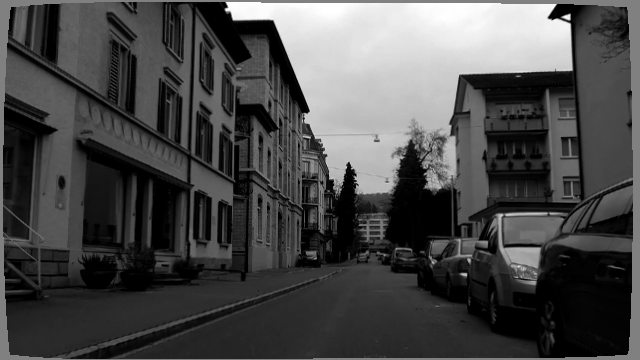
\includegraphics[width=.3\textwidth]{images/vespa_0014.png}\hfill
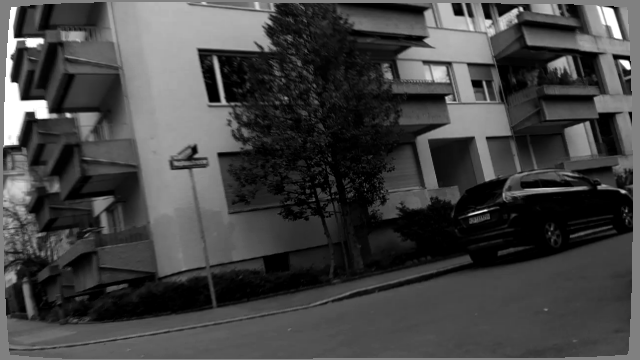
\includegraphics[width=.3\textwidth]{images/vespa_0292.png}\hfill
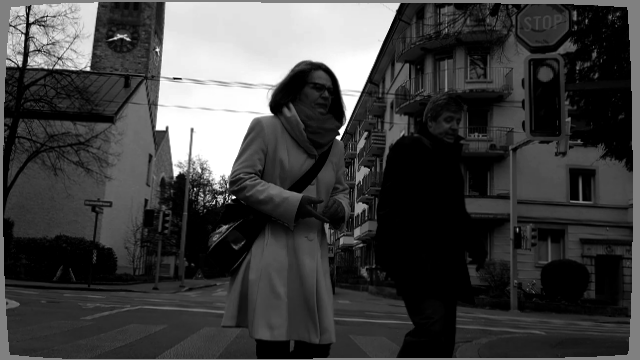
\includegraphics[width=.3\textwidth]{images/vespa_1072.png}
\captionsetup{justification=centering}
\caption{Frames from the Vespa data set: \\ \emph{1.} a normal frame, \emph{2.} slant while making turns, \emph{3.} pedestrians causing occlusions}
\label{fig:vespa}

\end{figure}

\section{Bundle Adjustment}
\label{bundle adjustment}
As mentioned in section ?? the stand-alone VO pipeline suffers from a significant amount of scale drift. This means that over the trajectory, the average scale of the displacements changes. \par
To counteract this drift, it is possible to use bundle adjustment (BA) which minimizes the reprojection error of landmarks over several views. In the pipeline, windowed BA is implemented. Every ?? frames, keypoints are adjusted and replaced over the last ?? frames. In order to ensure continuity, the adjusted point cloud and trajectory is translated such that the second last position (????? the second to last location??????) of the last segment coincides with first position of the newly adjusted segment. \par
Using BA, scale drift can be effectively counteracted as Fig. ?? a and b show. \par
Advantageous as BA in its current form may be, it is also very slow. This can be attributed to the fact that there are too many landmarks and poses for too few observations. In this case the Levenberg Marquart Optimization algorithm must be used leading to very poor performance. A way to improve this is to tune the tracking and triangulation parameters in a way to lose minimal matches over successive frames. This ensures that key points are observed several times before BA is executed. 

\section{Ground Truth Alignment and Error Analysis}
\label{simulation}

For a stable operation of the VO pipeline, optimized parameters must be chosen to control detection and matching of new key points, triangulation etc. To determine the optimal parameters, a suitable cost function must be defined to determine the quality of the resulting trajectories. To this end it is reasonable to compare the total error resulting after aligning the trajectory to the ground truth using the following formula:
\begin{equation}e_p = \underset{R,t,s}{\min} \sum_i (sR \cdot p_{GT, i} + t - p_{est, i})^2\end{equation}
$$e_r = \sum_i rotMatToRotVec(R^* \cdot R_{est,i} \cdot R_{GT, i}^T)^2$$
Where i is the index along the trajectory, $e_p$ is the positional error, $e_r$ is the rotational error, $p_{GT}$ and $R_{GT}$ are the ground truth position and rotation, $p_{est}$ and $R_{est}$ are the estimated position and rotation and $R^*$ is the argument for R when $e_p$ is minimal. The function rotMatToRotVec transforms the rotation matrix into a rotation vector of the form $\phi = \theta n$  Using these error metrics a detailed error analysis over the first ?? frames was done. More information on this can be found in section ??.

